\documentclass[border=10pt]{standalone}

\usepackage{tikz}
\usepackage{tikzsymbols}
\usetikzlibrary{calc,patterns,shapes.geometric}

\def\centerarc[#1](#2)(#3:#4:#5){\draw[#1] ($(#2)+({#5*cos(#3)},{#5*sin(#3)})$) arc (#3:#4:#5);}

\begin{document}
	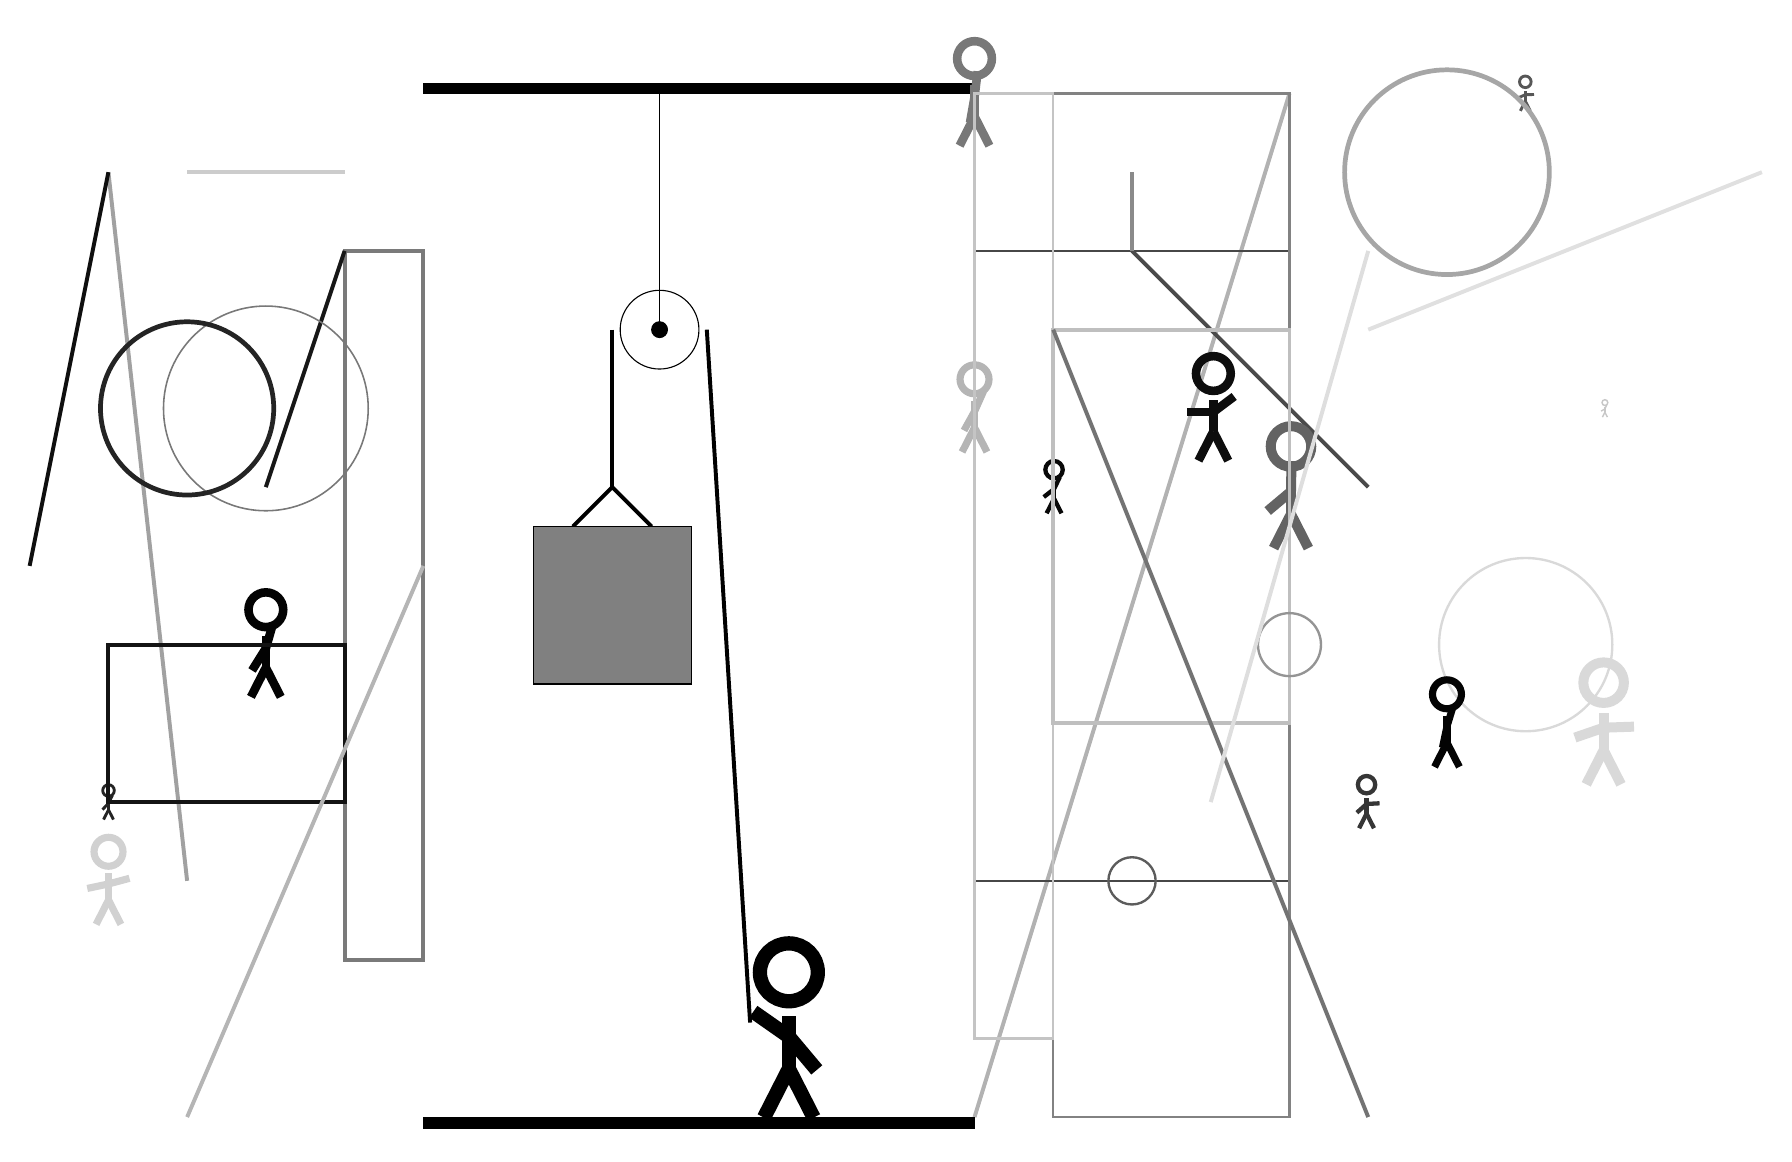
\begin{tikzpicture}
		%%%%% START %%%%%
		
		\draw[fill=black] (-2, 10) rectangle (5, 10.125);
		
		\draw (1, 7) circle (0.5);
		\draw[fill=black] (1, 7) circle (0.1);
		\draw (1, 10) -- (1, 7);
		
		\draw[line width=0.5mm] (-0.1, 4.5) -- (0.4, 5.0) -- (0.9, 4.5);
		\draw[fill=black!50] (-0.6, 4.5) rectangle (1.4, 2.5);
		
		\node[line width=0.6mm, color=black!53] at (5, 10) {\Strichmaxerl[6][80][83]};
		
		\draw[line width=0.5mm, color=black!52] (-3, -1) rectangle (-2, 8);
		\node[line width=0.2mm, color=black!29] at (5, 6) {\Strichmaxerl[5][61][66]};
		\draw[line width=0.5mm, color=black!91](-3, 8) -- (-4, 5);
		\draw[line width=0.5mm, color=black!37](-6, 9) -- (-5, 0);
		\node[line width=0.7mm, color=black!18] at (-6, 0) {\Strichmaxerl[5][12][15]};
		\draw [line width=0.2mm, color=black!53](-4, 6) circle (1.3);
		\draw[line width=0.5mm, color=black!30](5, -3) -- (9, 10);
		\draw[line width=0.2mm, color=black!72] (5, 0) rectangle (9, 8);
		\draw [line width=0.6mm, color=black!86](-5, 6) circle (1.1);
		\draw[line width=0.3mm, color=black!49] (6, -3) rectangle (9, 10);
		
		\node[line width=0.6mm, color=black!86] at (-6, 1) {\Strichmaxerl[2][46][64]};
		\draw [line width=0.3mm, color=black!15](12, 3) circle (1.1);
		\draw[line width=0.5mm, color=black!71](10, 5) -- (7, 8);
		\node[line width=0.5mm, color=black!66] at (12, 10) {\Strichmaxerl[2][24][1]};
		\draw[line width=0.3mm, color=black!23] (6, -2) rectangle (5, 10);
		\node[line width=0.2mm, color=black!95] at (8, 6) {\Strichmaxerl[6][0][37]};
		\node[line width=0.7mm, color=black!99] at (-4, 3) {\Strichmaxerl[6][58][74]};
		\node[line width=0.5mm, color=black!15] at (13, 2) {\Strichmaxerl[7][19][2]};
		\draw[line width=0.4mm, color=black!46] (7, 9) rectangle (7, 8);
		\draw[line width=0.5mm, color=black!92] (-3, 1) rectangle (-6, 3);
		
		\draw[line width=0.5mm, color=black!29](-2, 4) -- (-5, -3);
		\node[line width=0.3mm, color=black!61] at (9, 5) {\Strichmaxerl[7][40][89]};
		\draw[line width=0.5mm, color=black!12](10, 7) -- (15, 9);
		\draw[line width=0.5mm, color=black!94](-7, 4) -- (-6, 9);
		
		\node[line width=0.4mm, color=black!99] at (11, 2) {\Strichmaxerl[5][78][73]};
		\node[line width=0.2mm, color=black!97] at (6, 5) {\Strichmaxerl[3][38][64]};
		\draw[line width=0.5mm, color=black!25] (6, 7) rectangle (9, 2);
		\node[line width=0.3mm, color=black!79] at (10, 1) {\Strichmaxerl[3][42][3]};
		\draw[line width=0.5mm, color=black!55](6, 7) -- (10, -3);
		\draw [line width=0.6mm, color=black!35](11, 9) circle (1.3);
		\draw [line width=0.3mm, color=black!42](9, 3) circle (0.4);
		\node[line width=0.4mm, color=black!22] at (13, 6) {\Strichmaxerl[1][28][67]};
		\draw[line width=0.5mm, color=black!20](-5, 9) -- (-3, 9);
		\draw[line width=0.5mm, color=black!13](10, 8) -- (8, 1);
		\draw [line width=0.3mm, color=black!64](7, 0) circle (0.3);
		
		\draw[line width=0.5mm] (0.4, 7) -- (0.4, 5.0);
		\centerarc[line width=0.5mm](1, 7)(0:180:0.6);
		\draw[line width=0.5mm](1.6, 7) -- (2.15, -1.8);
		
		\node at (2.6, -1.9) {\Strichmaxerl[10][-35][-50]};
		
		\draw[fill=black] (-2, -3) rectangle (5, -3.15);
		
		%%%%% END %%%%%
	\end{tikzpicture}
\end{document}